\chapter{Modultest}
Ved modultests blev én funktionalitet testet isoleret. Det vil sige med så lidt påvirkning fra resten af systemet som muligt. Modultests blev udført før integrationstests, for at sikre individuel funktionalitet før sammensætning af alle komponenter. Modultests blev udført både for software-komponenter og hardware-komponenter.

\section{Software}
Til modultest af software er der gjort brug af white-box testing. Dette er gjort, da softwaren ligger tæt op ad hardwaren til kommunikationsbusserne, hvilket kræver teknisk viden om den interne struktur for både hardware og software.

\subsection{Opsummering}
\subsubsection{Wii-Nunchuck}
Dataoverførsel fra Wii-Nunchuck sker ved at PSoC0 først sender et \textit{handshake}, hvilket er en enkelt byte med værdien 0x00. Herefter kan PSoC0 aflæse Wii-Nunchuck tilstanden ved kontinuert at sende en byte med værdien \textit{??}, efterfulgt af den egentlig aflæsning. Det er altså disse to dele der skal testes på.

For flere tekniske detaljer, samt billeder af målingerne, refereres til \textbf{DOKUMENTATION \#ref}

Tabel \ref{table:modulTestNunchuckHandShake} og \ref{table:modulTestNunchuckReading} præsenterer modultest resultaterne for Wii-Nunchuck.

\begin{table}[H]
	\centering
	\begin{tabular}{ll}
		\hline
		Forventet Resultat & \begin{tabular}[c]{@{}l@{}}På I2C Bussen måles et \textit{ACKNOWLEDGE} fra Wii-Nunchuck \\ slaven når den får tilsendt et handshake fra PSoC0. Det skal \\ desuden kunne ses at en byte med værdien 0x00 modtages \\ af Wii-Nunchuck. \end{tabular} \\
		\rowcolor[HTML]{CBCEFB} 
		Egentlig Resultat  & \begin{tabular}[c]{@{}l@{}}Et \textit{ACKNOWLEDGE} blev målt som forventet, \\ og handshake byten med værdi 0x00 blev modtaget korrekt. \end{tabular}                                       \\ \hline
	\end{tabular}
	\caption{Modultest af Wii-Nunchuck Handshake}
	\label{table:modulTestNunchuckHandShake}
\end{table}

\begin{table}[H]
	\centering
	\begin{tabular}{ll}
		\hline
		Forventet Resultat & \begin{tabular}[c]{@{}l@{}}På I2C bussen måles en aflæsning af bytes fra Wii-Nunchuck\\ slaven.\end{tabular}                \\
		\rowcolor[HTML]{CBCEFB} 
		Egentlig Resultat  & \begin{tabular}[c]{@{}l@{}}På målingen af I2C bussen ses det at bytes bliver aflæst fra\\ Wii-Nunchuck slaven.\end{tabular} \\ \hline
	\end{tabular}
	\caption{Modultest af Wii-Nunchuck Data Aflæsning}
	\label{table:modulTestNunchuckReading}
\end{table}

Det kan på tabel \ref{table:modulTestNunchuckHandShake} og \ref{table:modulTestNunchuckReading} ses at de egentlige resultaterne stemte overens med de forventede.

\subsubsection{I2C Kommunikationsprotokol}
I2C Kommunikationsprotokollen beskrevet i afsnit \ref{afsnit:I2CProtokol} blev modultestet ved to tests. Den første test er til for at verificere at kommandotyper bliver overført på I2C bussen i korrekt format. Den anden test er til for at verificere at modtaget I2C data fortolkes korrekt af software på PSoC0.

\begin{table}[H]
	\centering
	\begin{tabular}{ll}
		\hline
		Forventet Resultat & \begin{tabular}[c]{@{}l@{}}På I2C Bussen måles kommandotypen NunchuckData \\i korrekt format.\end{tabular} \\
		\rowcolor[HTML]{CBCEFB} 
		Egentlig Resultat  & \begin{tabular}[c]{@{}l@{}}Målingen af I2C bussen viste kommandotypen \\ NunchuckData i korrekt format.  \end{tabular}                                       \\ \hline
	\end{tabular}
	\caption{Modultest af kommandotype på I2C Bussen}
	\label{table:modulTestCommandFormat}
\end{table}

\begin{table}[H]
	\centering
	\begin{tabular}{ll}
		\hline
		Forventet Resultat & \begin{tabular}[c]{@{}l@{}} \end{tabular} \\
		\rowcolor[HTML]{CBCEFB} 
		Egentlig Resultat  & \begin{tabular}[c]{@{}l@{}}  \end{tabular}                                       \\ \hline
	\end{tabular}
	\caption{Modultest af kommandofortolkningssoftware}
	\label{table:modulTestI2CData}
\end{table}

\subsubsection{SPI Kommunikationsprotokol}

\subsubsection{Rotationsdetektor}
\begin{table}[H]
	\centering
	\begin{tabular}{|l|c|c|}
		\hline
		\textbf{Indgangssignal} & \textbf{Forventet PWM} & \textbf{Målt PWM} \\ \hline
		0V                      & Ja                     & Ja                \\ \hline
		1400mV                  & Ja                     & Ja                \\ \hline
		1500mV                  & Ja                     & Ja                \\ \hline
		1600mV                  & Nej                    & Ja                \\ \hline
		2,2V                    & Nej                    & Ja                \\ \hline
		2,3V                    & Nej                    & Nej               \\ \hline
		5V                      & Nej                    & Nej               \\ \hline
	\end{tabular}
	\caption{Modultest af ADC}
	\label{my-label}
\end{table}

\subsection{Modultest af Wii-Nunchuck}
På PSoC0 er der software til aflæsning af Wii-Nunchuck input data. Følgende afsnit beskriver test af dette software.

Aflæsning af Wii-Nunchuck sker i to skridt, som begge verificeres ved modul test. Først skal der sendes et \textit{Handshake} fra PSoC0 til Wii-Nunchuck for at initialisere data udveksling, og herefter sker data udveksling hver gang PSoC0 sender en anmodning om det. Disse to skridt modultestes her.

\textbf{Test af Wii-Nunchuck Handshake}

\textbf{Test af data udveksling mellem PSoC0 og Wii-Nunchuck} 

PSoC0 blev programmeret til kontinuert aflæsning af Wii-Nunchuck. For at verificere data udveksling mellem PSoC0 og Wii-Nunchuck blev I2C bussen målt ved brug af Logic Analyzer fra Analog Discovery.

Data udveksling sker i to skridt. Først sender PSoC0 en byte med værdien 0 (0x00 i hexadecimal). Herefter sker den faktiske aflæsning, PSoC0 aflæser Wii-Nunchuck. Begge skridt testes her.

\textbf{Afsendelse af 0x00 byte}

Den første forventede I2C besked er en \textit{0x00} byte fra PSoC0 for at starte en ny aflæsning. På figur \ref{fig:NunchuckWriteValues} ses aflæsningen af I2C bussen på tidspunktet hvor anmodningen til Wii-Nunchuck bliver udført. Dette er en tidslinje læst fra ventre til højre.

\begin{figure}[H]
	\centering
	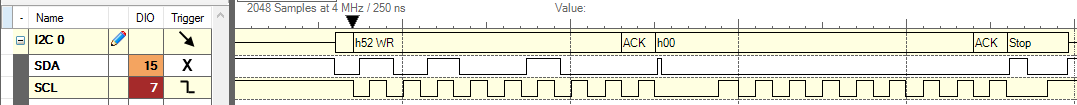
\includegraphics[width=\textwidth]{Test/images/writerequest}
	\caption{}
	\label{fig:NunchuckWriteValues}
\end{figure}

Det kan på figur \ref{fig:NunchuckWriteValues} ses at den første besked der måles er af typen "WR" (Write) til addressen 0x52 (Wii-Nunchuck I2C Slave Addressen). Hertil kommer et tilhørende \textit{ACK} (Acknowledge) fra Wii-Nunchuck. Til sidst sendes dataen Ox00 efterfulgt af at ACK fra Wii-Nunchuck. Til sidst afsluttes I2C transaktionen ved "Stop".

Det kan altså konkluderes at målingen er i overensstemmelse med forventningen om at en 0x00 byte skal sendes til Wii-Nunchuck for opstart af dataudveksling.

\textbf{Aflæsning af Wii-Nunchuck}

Efter vellykket afsendelse af 0x00 byten sker den egentlige aflæsning af Wii-Nunchuk input dataen.

Her forventes en række beskeder indeholdende 

På figur \ref{fig:NunchuckReadValues} ses I2C beskederne der bliver udvekslet mellem PSoC0 og Wii-Nunchuck efter vellykket Wii-Nunchuck Handshake. 

\begin{figure}[H]
	\centering
	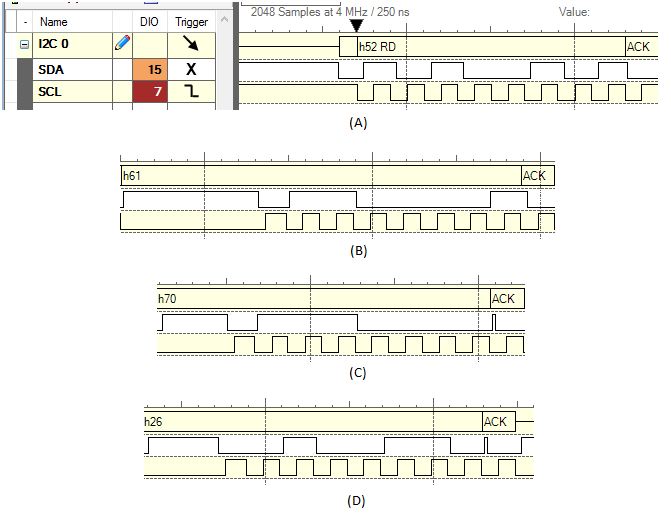
\includegraphics[width=\textwidth]{Test/images/readvaluesEdited.png}
	\caption{Tidslinje af aflæste I2C beskeder af PSoC0 fra Wii-Nunchuck}
	\label{fig:NunchuckReadValues}
\end{figure}

\subsection{SPI Protokol}
Devkittet kommunikerer over en SPI bus. Kommunikationen følger SPI kommunikations protokollen, som er beskrevet i afsnit \ref{afsnit:spiprotokol}. Dette afsnit beskriver test af denne protokol.

\subsubsection{SPI Bus Test}
Test af SPI bussen udføres i to dele. Første del af testen udføres ved at sende kommandotypen for start af SPI test i terminalen, og derefter verificere den sendte data vha. Analog Discovery. Den anden del af testen, er at aflæse returbeskeden på bussen med Analog Discovery. Målet med denne test, er at læse kommandotypen "SPI\_OK", der indikerer en successful aflæsning af SPI-slaven.  På figur \ref{figure:SpiTestSetup} ses test opsætningen. Devkit8000, PSoC0s SPI-bus og Analog Discovery  er forbundet til hinanden igennem fumlebrættet. PSoC0 og PSoC1's I2C-forbindelser forbindes til nunchucken igennem fumlebrættet, adskilt fra SPI-forbindelserne.


\begin{figure}[H]
	\centering
	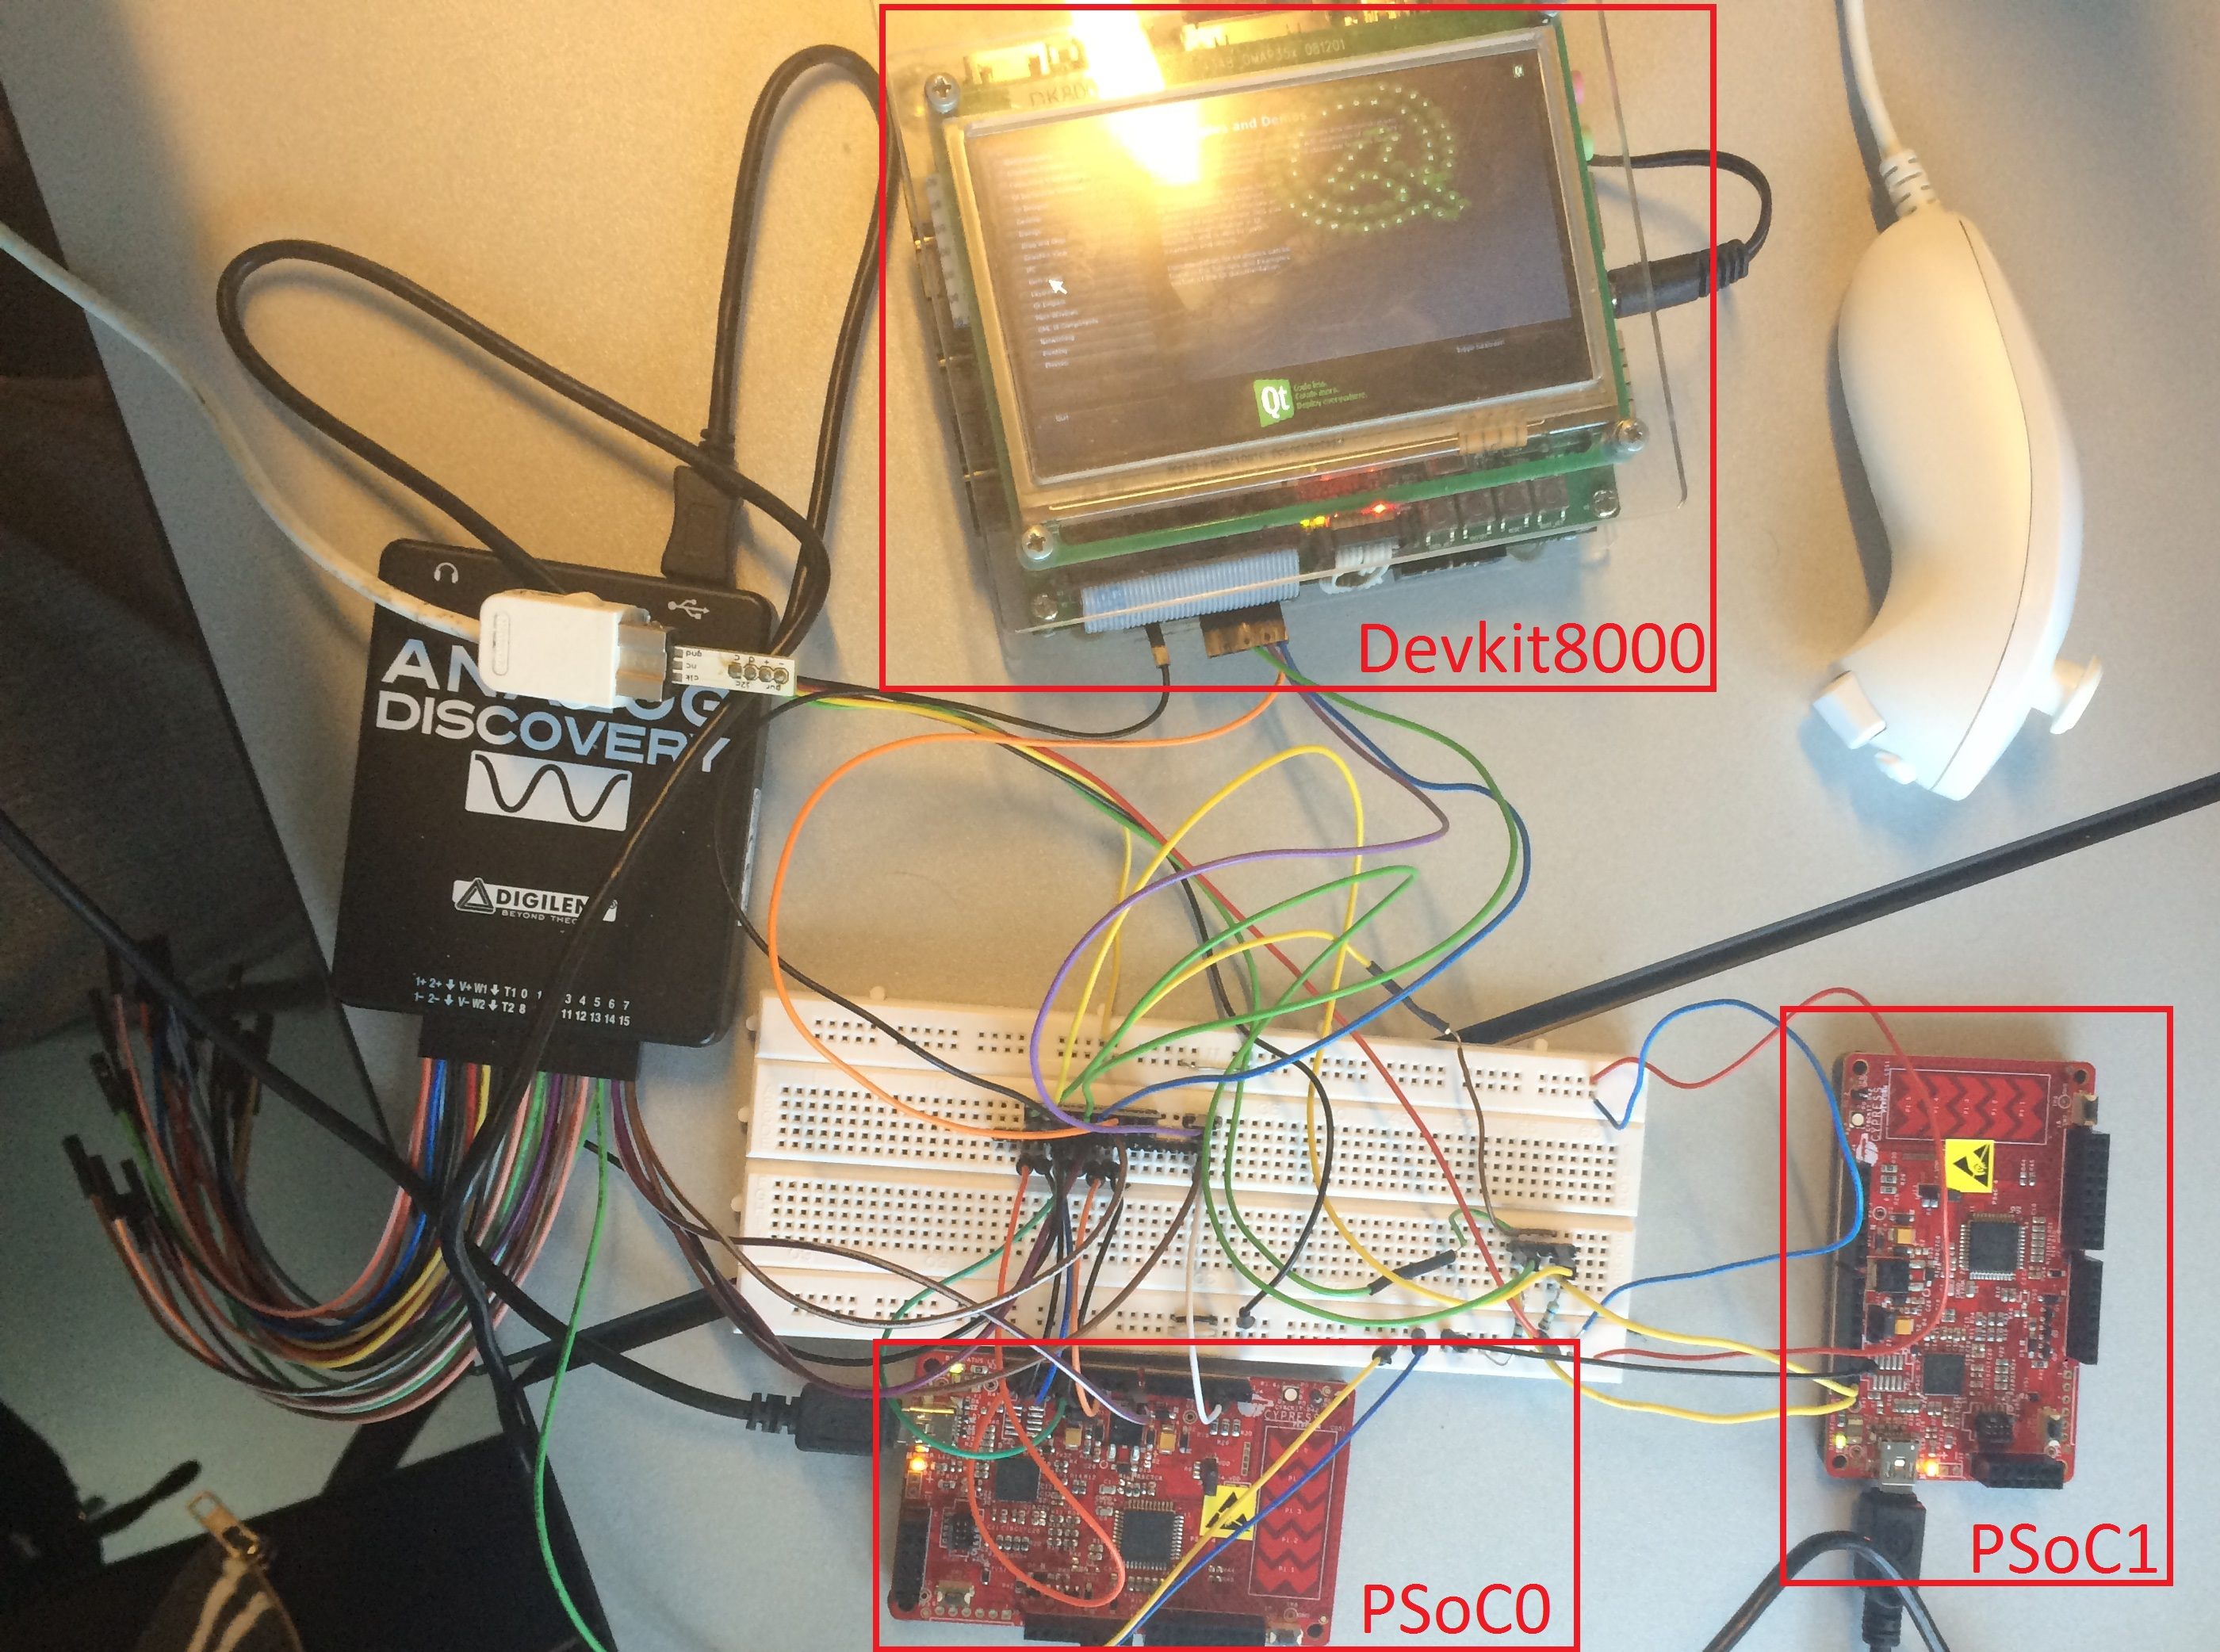
\includegraphics[width=\textwidth]{Test/images/SPItest/SpiTestSetup}
	\caption{Opsætning for SPI-test}
	\label{figure:SpiTestSetup}
\end{figure}


I testen afsendes SPI test kommandotypen, som har værdien 0xF1 jf. tabel \ref{tabel:spiKommandoType}. For at verificere, at kommandotypen er sendt ud på SPI-bussen korrekt, blev Analog Discovery's 'Logic Analyzer' brugt til at aflæse SPI-bussen. Det var forventet at 0xF1 blev aflæst på bussen. Det afmålte resultat stemte overens med det forventede. Målingen ses på figur \ref{fig:SPItestkommandotype}. 

\begin{figure}[H]
	\centering
	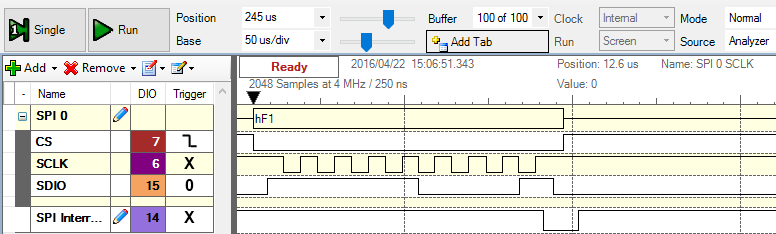
\includegraphics[width=\textwidth]{Test/images/SPItest/SPItestkommandotype}
	\caption{Måling af kommandotype for start SPI test}
	\label{fig:SPItestkommandotype}
\end{figure}

Hvis SPI-kommunikationen fungerer korrekt, er det forventet at der aflæses 0xD1 på SPI-bussen, da dette betyder 'SPI\_OK' jf. tabel \ref{tabel:spiKommandoType}. Måling af returbeskeden ses på figur \ref{fig:SPItestSPIOK}.

\begin{figure}[H]
	\centering
	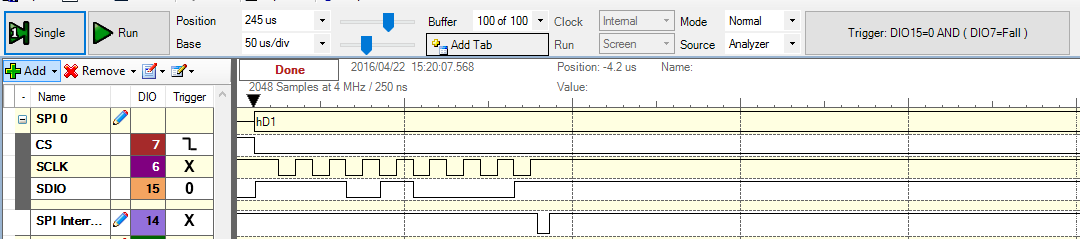
\includegraphics[width=\textwidth]{Test/images/SPItest/SPItestSPIOK1}
	\caption{Måling af returbesked for start SPI test} 
	\label{fig:SPItestSPIOK}
\end{figure}

På figur \ref{fig:SPItestSPIOK} ses at returbeskeden har den forventede værdi 0xD1, som indikerer at SPI bus testens første del er gennemført uden fejl.

Ud fra testenes resultater kan det konkluderes at implementeringen af SPI protokollen fungerer efter hensigten.



\subsection{I2C Protokol}
PSoC0 og PSoC1 kommunikerer over en I2C bus via I2C protokollen beskrevet i afsnit \ref{afsnit:I2CProtokol}. Dette afsnit beskriver test af denne protokol. Følgende test tager udgangspunkt i kommandotypen \textit{NunchuckData} beskrevet i tabel \ref{table:I2CKommandoer}).

\subsubsection{Test af NunchuckData kommandotype} 

Testen blev udført i to dele. I første del måles I2C bussen ved brug af Analog Discovery's Logic Analyzer; for at verificere at den forventede kommandotype bliver overført via bussen. Anden del verificerer at den overførte data er modtaget korrekt via PSoC Creator's debugger.

\subsubsection{NunchuckData kommandotype test del 1}

I testen afsendes, som nævnt i afsnittets indledning, kommandotypen NunchuckData. Som vist i tabel \ref{table:I2CKommandoer} har denne kommandotype ID'et 0xA2, hvor de efterfølgende 3 data bytes indeholder input dataen fra Wii-Nunchuck.

Det forventede resultat af målingen er at første byte er kommandoentypens ID, som har værdien 0x2A. Kommandoens data - de efterfølgende bytes - verificeres først i anden del, disse indgår altså ikke i følgende måling. 

Målingen ses på figur \ref{fig:NunchuckDataCommand}.

\begin{figure}[H]
	\centering
	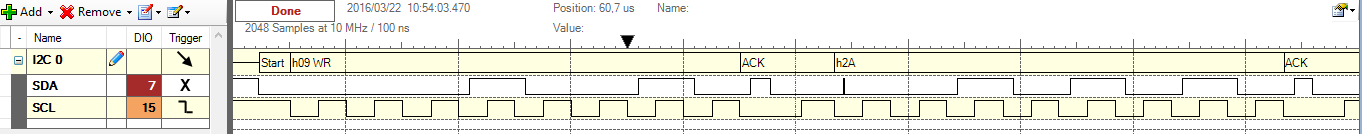
\includegraphics[width=1.2\textwidth]{Test/images/ShowsNunchuckDataCommand.png}
	\caption{Tidslinje af målt I2C kommandotype}
	\label{fig:NunchuckDataCommand}
\end{figure}

Det kan ses på figur \ref{fig:NunchuckDataCommand} at I2C overførslen starter med en I2C \textit{write}, som får et successfuldt acknowledge fra slaven PSoC1. Herefter kan det ses at den næste byte der sendes har værdien 0x2A. Denne byte er kommandoentypens ID, og er altså som forventet 0x2A.

Det kan altså verificeres at kommandoen overføres via I2C bussen. Dataens integritet er dog ikke inkluderet i denne del, og testes i del 2.

\subsubsection{NunchuckData kommandotype test del 2}
For at verificere integriteten af den data der sendes mellem PSoC0 og PSoC1, bruges PSoC Creators indbyggede debugger. Igen er det kommandotypen NunchuckData der sendes mellem de to enheder, hvor de medfølgende data bytes fortolkes.

Testen gennemføres ved at fortolke den modtagne data tre gange, hvor nunchucken er i forskellige tilstande (hvilken retning det analoge stik er trykket) i hver test. Værdierne sammenlignes de forventede standardværdier som ses i tabellen på side 3 i \cite[I2C Interface with Wii Nunchuck]{nunchuck}. Da testene kun er fokuserede på, hvilken retning den analoge stick er presset, er det altså kun receivedDataBuffer[1] (den analoge stick x-akse) og receivedDataBuffer[2] (den analoge pinds y-akse) der er relevante for testen. Når den analoge stick er presset til venstre, forventes det ifølge tabel \ref{tabel:WiiNunchuckStickPositioner} at receivedDataBuffer[1] er lig 0x1E og receivedDataBuffer[2] er 0x7B. Når den analoge stick er presset op, forventes det at receivedDataBuffer[1] er 0x7E og receivedDataBuffer[2] er 0xDF. Når der ikke er noget input på Nunchucken forventes det at receivedDataBuffer[1] er 0x7E og receivedDataBuffer[2] er 0x7B. Målingerne for testene kan ses på figur \ref{fig:I2CProtocolReadNoInput}, \ref{fig:I2CProtocolReadLeftAnalog} og \ref{fig:I2CProtocolReadUpAnalog}.

\begin{figure}[H]
	\centering
	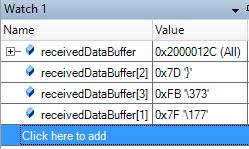
\includegraphics[width=.5\textwidth]{Test/images/I2CProtocolReadNoInput.png}
	\caption{Afmåling af modtager-buffer på PSoC1 efter at have modtaget "NunchuckData" kommando typen. Intet input på Nunchuck'en}
	\label{fig:I2CProtocolReadNoInput}
\end{figure}

\begin{figure}[H]
	\centering
	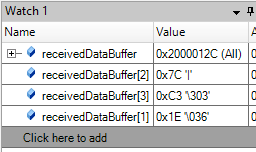
\includegraphics[width=.5\textwidth]{Test/images/I2CProtocolReadLeftAnalog.png}
	\caption{Afmåling af modtager-buffer på PSoC1 efter at have modtaget "NunchuckData" kommando typen. Den analoge stick er presset til venstre på Nunchuck'en}
	\label{fig:I2CProtocolReadLeftAnalog}
\end{figure}

\begin{figure}[H]
	\centering
	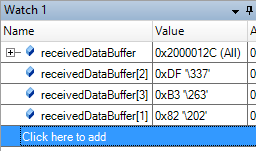
\includegraphics[width=.5\textwidth]{Test/images/I2CProtocolReadUpAnalog.png}
	\caption{Afmåling af modtager-buffer på PSoC1 efter at have modtaget "NunchuckData" kommando typen. Den analoge stick er presset frem på Nunchuck'en}
	\label{fig:I2CProtocolReadUpAnalog}
\end{figure}

På figur \ref{fig:I2CProtocolReadLeftAnalog} ses afmålingen af modtager-bufferen når Nunchuckens analoge stick er presset helt til venstre. ReceivedDataBuffer[1] blev aflæst til 0x1E og receivedDataBuffer[2] blev aflæst til 0x7C. ReceivedDataBuffer[1] stemmer overens med forventningerne. ReceivedDataBuffer[2] har en lille afvigelse (oversat til decimaltal blev der målt 124, hvor der forventes 123). Denne afvigelse kan skyldes, at det analoge stick ikke blev presset direkte til venstre, men at den også er blevet presset en smule frem under målingen.

På figur \ref{fig:I2CProtocolReadUpAnalog} ses afmålingen af modtager-bufferen når Nunchuckens analoge stick er presset frem. ReceivedDataBuffer[1] blev aflæst til 0x82, hvor det var forventet 0x7E. Dette er en afvigelse fra de forventede resultater med 4, og kan skyldes at det analoge stick ikke var helt centreret idét den blev presset frem under målingen. ReceivedDataBuffer[2] blev aflæst til 0xDF, hvilket stemmer overens med de forventede målinger.

På figur \ref{fig:I2CProtocolReadNoInput} ses afmålingen af modtager-bufferen når der ikke er noget brugerinput på nunchuckens analoge stick. ReceivedDataBuffer[1] blev aflæst til 0x7F, hvor det forventede resultat var 0x7E. Denne afvigelse kan skyldes at det analoge stick ikke stod helt i midten under målingen (Det analoge stick er lidt "løs" og kan defor godt finde hvile i en position der ikke er fuldt centreret). ReceivedDataBuffer[2] blev aflæst til 0x7D, hvor det forventede resultat var 0x7B. Igen kan denne afvigelse skyldes at det analoge stick ikke var i centrum under målingen.

Ud fra testen kan det konkluderes at implementeringen af I2C-protokollen fungerer efter hensigten.

\section{Hardware}
\subsection{H-bro} 

\textbf{Formål} \newline
Formålet med denne test er at vise at en motor kan styres i begge retninger med H-broen.\newline

\noindent \textbf{Opstilling}

\begin{figure}[H]
	\centering
	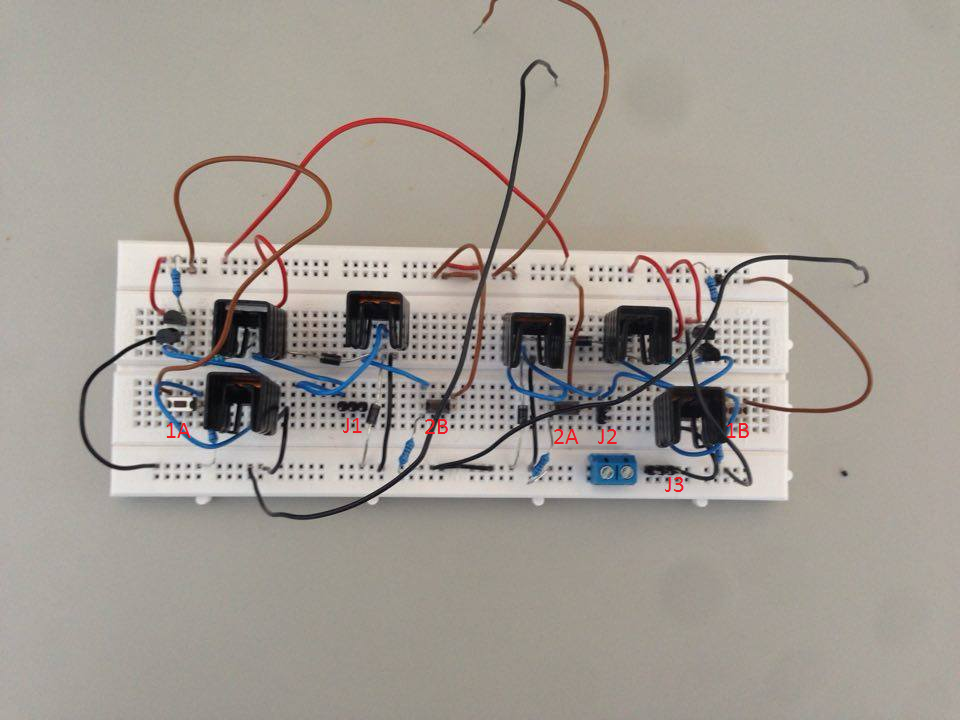
\includegraphics[width=\textwidth]{test/images/testhbroopst}
	\caption{Opstilling af H-bro på fumlebræt}
\end{figure}

\begin{table}[H]
	\centering
	\label{hbro}
	\begin{tabular}{|l|l|}
		\hline
		\textbf{Element} & \textbf{Beskrivelse}                   \\ \hline
		J1, J2           & Output Pins                            \\ \hline
		J3               & Stel Pin                               \\ \hline
		1a, 2a           & Knapper til at styre motor til højre   \\ \hline
		1b, 2b           & Knapper til at styre motor til venstre \\ \hline
		Sorte ledninger  & Stel                                   \\ \hline
		Røde ledninger   & 9V                                     \\ \hline
		Brune ledninger  & 5V                                     \\ \hline
		Blå ledninger    & Interkomponente forbindelser           \\ \hline
	\end{tabular}
		\caption{Elementer i testopstillingen}
\end{table}

\noindent Til test af H-broens motorstyring i begge retninger blev to oscilloskop kanaler forbundet til output pin J1 og J2, samt oscilloskopenes stel til J3. Fumlebrættet forsynes med 9V, 5V og stel fra en spændingskilde. 

\noindent Testen blev udført i to dele. Først testes H-broen i højre omdrejningsretning ved at trykke på 1a og 2a, derefter i venstre omdrejning ved at trykke 1b og 2b. \newline

\noindent \textbf{Forventet resultat} \newline
I første del af modultesten forventes det at når 1a og 2a blev nedtrykket vil den blå kurve stige til 9V samt den orange kurve vil falde til 0V. Ved anden del af testen forventes det at når 1b og 2b blev nedtrykket vil den orange kurve stige til 9V samt den blå kurve falde til 0V. \newline

\noindent \textbf{Opnået resultat}

\begin{figure}[H]
	\centering
	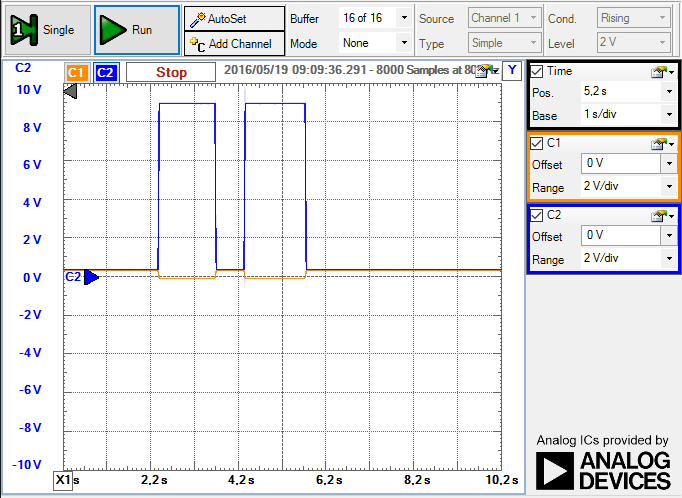
\includegraphics[width=\textwidth]{test/images/hbromob}
	\caption{Modultest for højre omdrejningsretning}
		\label{figure:hbrob}
\end{figure}

 \noindent Som det fremgår af figur \ref{figure:hbrob}, ses det at, når 1a og 2a nedtrykkes får det blå retningssignal forbindelse til stel og dermed trækker denne alt spændingen og stiger til 9V. Da alt spænding trækkes af det blå retningssignal, bliver det orange retningssignal groundet. Dermed kan motoren styres via H-broen i højre omdrejningsretning. 

\begin{figure}[H]
	\centering
	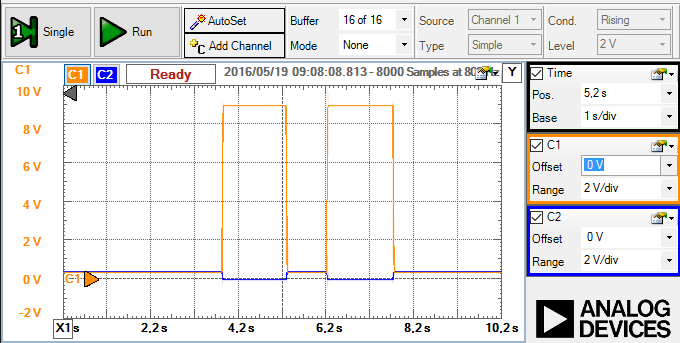
\includegraphics[width=\textwidth]{test/images/hbromoo}
	\caption{Modultest for H-bro, orange går høj}
	\label{figure:hbroo}
	
\end{figure}

Ved anden del af modultesten nedtrykkes 1b og 2b. På figur \ref{figure:hbroo} ses resultatet af dette. Det observeres at knappene nedtrykkes får det orange retningssignal forbindelse til stel og stiger til 9V, samt at det blå retningssignal falder til 0V. Dermed er det bevist at motoren kan styres vi H-broen i venstre omdrejningsretning. 

Ud fra disse to test kan det konkluderes at en motor kan styres i begge omdrejningsretninger via H-broen. Fra figurene \ref{figure:hbrob} og \ref{figure:hbroo} kan det også observeres at der ikke fremkommer støj, når retningssignalerne stiger til 9V, dermed vil der ikke være forstyrrende elementer der kommer til at påvirke styringen af motoren.
  

\subsection{Rotationsbegrænsning}
\noindent \textbf{Formål} \newline
\noindent Formålet med denne test er at bevise at motoren ikke kan køre ud over de ydergrænser, men kan bevæge sig frit i det tilladte interval. \newline

\noindent \textbf{Opstilling}
\begin{figure}[H]
	\centering
	\includegraphics[width=\textwidth]{test/images/ModultestADC/opstilADC}
	\caption{Testopstilling for rotationsbegrænsning}
\end{figure}

\noindent \textbf{Bemærkning: }Ved denne testopstilling er potentiometeret ikke fastsat til motoren, dermed følger output spændingen ikke motorens rotationer. Denne test bruges til at bevise at retningssignaler blokeres, når potentiometeret bevæges udover de tilladte grænser. Dette gøres manuelt. 

\begin{table}[H]
	\centering
	\label{table:RBelements}
	\begin{tabular}{|l|l|}
		\hline
		\textbf{Element} & \textbf{Beskrivelse}                              \\ \hline
		1                & Potentiometer                                     \\ \hline
		2                & H-bro                                             \\ \hline
		3                & PSoC1                                             \\ \hline
		4                & Wii-Nunchuck                                      \\ \hline
		5                & PSoC0                                             \\ \hline
		6                & Print med pull-up modstande til I2C kommunikation \\ \hline
		Sorte ledninger  & Stel                                              \\ \hline
		Røde ledninger   & 5V                                                \\ \hline
		Gule ledninger   & Data linjer mellem moduler                        \\ \hline
		Grønne ledninger  & Clock signal                                      \\ \hline
	\end{tabular}
	\caption{Elementer i testopstillingen}
\end{table}

Test af rotationsbegrænsning blev udført i tre dele. I første del testes om motoren kan styres i begge retninger når outputspændingen fra potentiometret ligger mellem 915mV og 2000mV. I anden del testes der for at retningssignalet til venstre blokeres når potentiometerets outputspænding overstiger 2000mV. I tredje del testes der for at retningssignalet til højre blokeres når potentiometerets outputspænding falder under 915mV. 

Til at monitorere outputspændingen fra potentiometeret er et Analog Discovery tilsluttet til dens udgange gennem et fumlebræt. Til at for at aflæse værdier fra AD converteren sættes PSoC1 i debug mode. Resultater verficeres visuelt. \newline

\noindent \textbf{Forventet resultat} \newline
Første del: Potentiometeret indstilles til midterposition. Det observeres at motoren kan roteres i begge retninger. \newline
Anden del: Potentimetret indstilles til at have den størst mulig modstandsværdi. Det observeres at motoren kun kan roteres til højre. \newline
Tredje del: Potentiometret indstilles til at have lavest mulig modstandsværdi. Det observeres at motoren kun kan roteres til venstre. \newline

\noindent Da ADC'en har en referencespænding på 3.3V og outputtet af potentiometret er mellem 0V-5V er foholdet givet ved:
\begin{equation}
\frac {5V} {3.3V}= 1.515
\end{equation}
Dermed forventes der et tilnærmelsesvis forhold mellem ADC'ens og potentiometrets output. \newline

\noindent \textbf{Opnået resultat}
\begin{figure}[H]
	\centering
	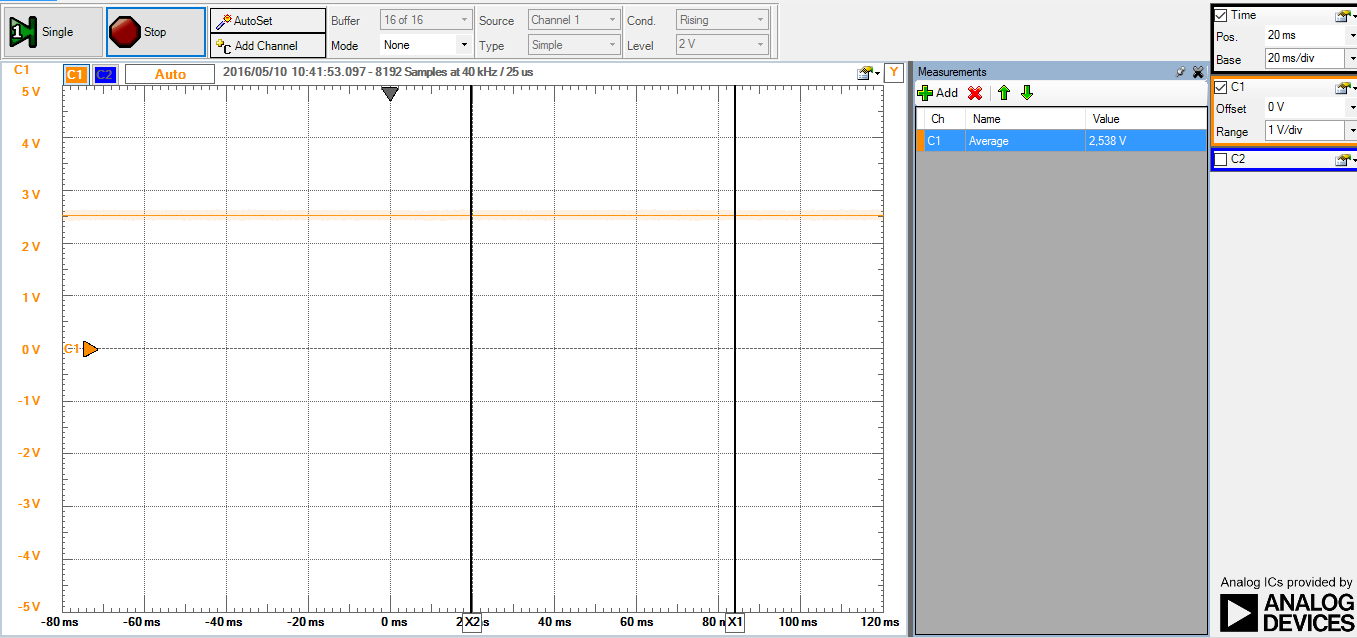
\includegraphics[width=\textwidth]{test/images/ModultestADC/2538Vanalog}
	\caption{Første del: Potentiometer output 2538mV}
	\label{figure:analogmid}
\end{figure}
\begin{figure}[H]
	\centering
	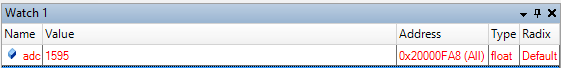
\includegraphics[width=\textwidth]{test/images/ModultestADC/mellemDebug}
	\caption{Første del: ADC output 1595mV}
	\label{figure: ADCmid}
\end{figure}

\noindent Som det fremgår på figur \ref{figure:analogmid} er output spændingen af potentiometeret 2538mV og på figur \ref{figure: ADCmid} ses det at outputspændingen af ADC’en har en værdi på 1595mV. Tages der hensyn til det førnævnte forhold, ses det at den forventede outputspænding er:
\begin{equation}
1595mV * 1.515 = 2416mV
\end{equation}
Da den faktiske spænding fra potentiometeret 2538mV stemmer det faktiske resultat overens med det forventede resultat. Det observeres at motoren kan styres i begge retninger.

\begin{figure}[H]
	\centering
	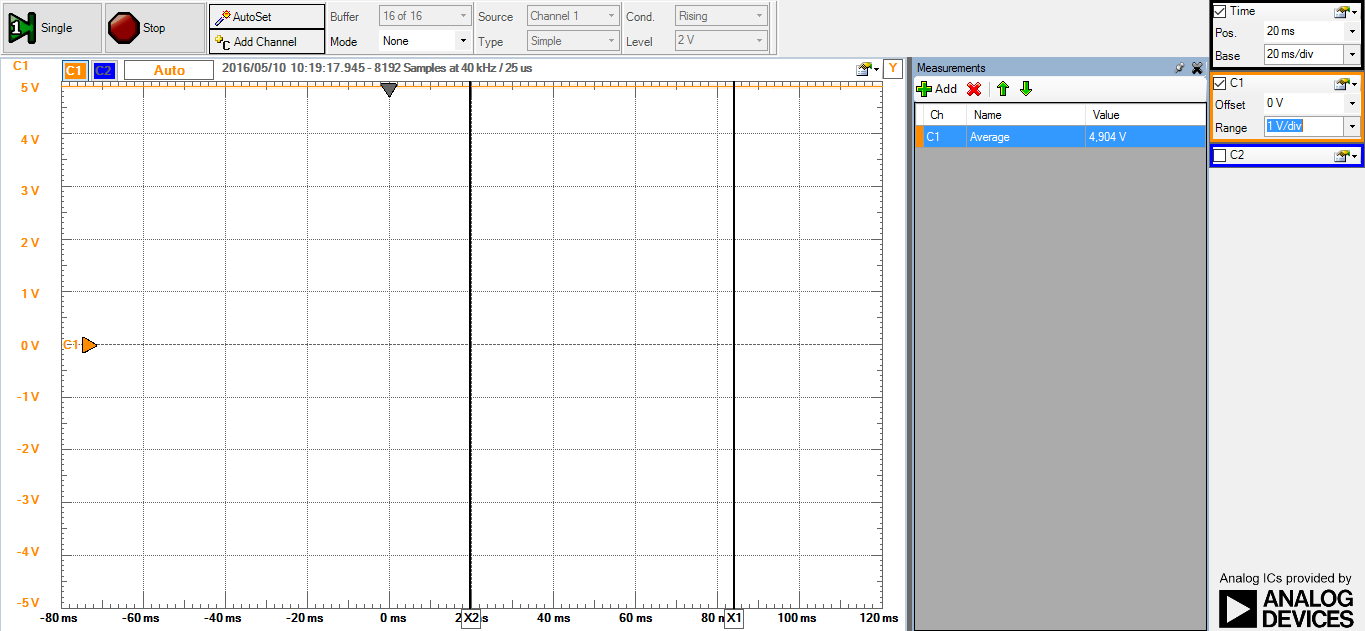
\includegraphics[width=\textwidth]{test/images/ModultestADC/4904mVanalog}
	\caption{Anden del: Potentiometer output 4904mV}
	\label{figure:analoghoj}
\end{figure}
\begin{figure}[H]
	\centering
	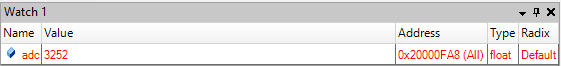
\includegraphics[width=\textwidth]{test/images/ModultestADC/opDebug}
	\caption{Anden del: ADC output 3252mV}
	\label{figure: ADChoj}
\end{figure}
\noindent Som det fremgår på figur \ref{figure:analoghoj} er output spændingen af potentiometeret 4904mV og på figur \ref{figure: ADChoj} ses det at outputspændingen af ADC’en har en værdi på 3252mV. Tages der hensyn til det førnævnte forhold, ses det at den forventede outputspænding er:
\begin{equation}
3252mV * 1.515 = 4926mV
\end{equation}
Da den faktiske spænding fra potentiometeret 4904mV stemmer det faktiske resultat overens med det forventede resultat. Det observeres at motoren kun kan styres i højre.

\begin{figure}[H]
	\centering
	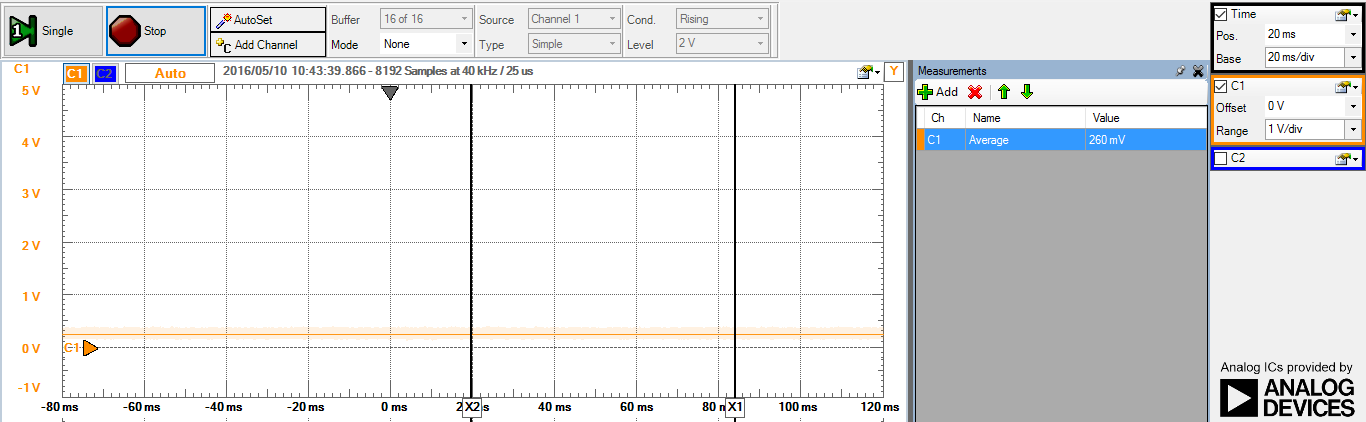
\includegraphics[width=\textwidth]{test/images/ModultestADC/260mVanalog}
	\caption{Tredje del: Potentiometer output 260mV}
	\label{figure:analoglav}
\end{figure}
\begin{figure}[H]
	\centering
	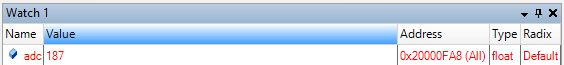
\includegraphics[width=\textwidth]{test/images/ModultestADC/nedDebug}
	\caption{Tredje del: ADC output 187mV}
	\label{figure: ADClav}
\end{figure}

\noindent Som det fremgår på figur \ref{figure:analoglav} er output spændingen af potentiometeret 260mV og på figur \ref{figure: ADClav} ses det at outputspændingen af ADC’en har en værdi på 187mV. Tages der hensyn til det førnævnte forhold, ses det at den forventede outputspænding er:
\begin{equation}
187mV * 1.515 = 280.5mV
\end{equation}
Da den faktiske spænding fra potentiometeret 260mV stemmer det faktiske resultat overens med det forventede resultat. Det observeres at motoren kun kan styres til venstre.

Ud fra disse tre deltests kan det konkluderes at rotationsbegrænsningen fungerer efter hensigten.


\subsection{Rotationsdetektor}
Der er udført en række modultests af rotationsdetektoren. Først er der en beskrivelse af testen, der skulle teste de forskellige dele i rotationsdetektorkredsløbet, både mens fotodioden modtager et lyssignal fra LED'en, og når den ikke gør. Herefter følger en beskrivelse af modultesten af det båndpasfilter, der indgår i rotationsdetektoren og til sidst er der en beskrivelse af modultesten af motorens PWM-signal. 

På figur \ref{fig:målepunkter} ses, hvor der er målt for at teste rotationsdetektoren. 

\begin{figure}[H]
	\centering
	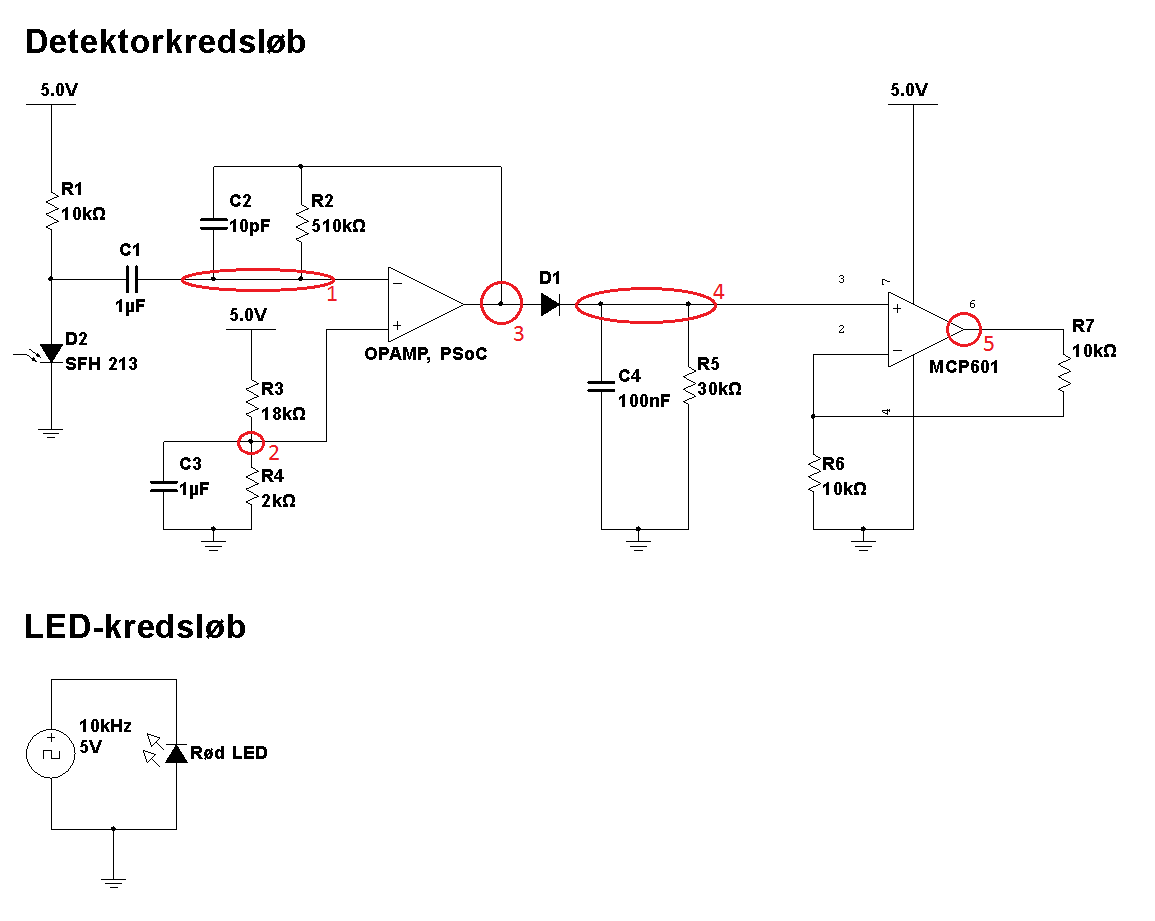
\includegraphics[width=\textwidth]{Test/images/rotationsdetektor_maalepunkter}
	\caption{Målepunkter på rotationsdetektor}
	\label{fig:målepunkter}
\end{figure}

I tabel \ref{dioderIkkeSe} ses resultaterne fra modultesten af rotationsdetektoren, når fotodioden ikke får noget lyssignal. Det ses, at det virtuelle nul fra spændingsdeleren ligger på 0,4V, og at forstærkeren fordobler signalet, hvilket var meningen. 

\begin{table}[H]
	\centering
	\begin{tabular}{|l|l|c|c|}
		\hline
		\textbf{Knudepunkt}		& \textbf{Målested}       & \textbf{Forventet resultat} & \textbf{Målt resultat} \\ \hline
		1						& Virtuelt 0              & 0,5V                        & 0,4V                   \\ \hline
		2						& Spændingsdeler          & 0,5V                        & 0,45V                  \\ \hline
		3						& Udgang på OpAmp på PSoC & 0,5V                        & 0,4V                   \\ \hline
		4 						& Envelope detector       & 0,5V                        & 0,4V                   \\ \hline
		5 						& Udgang på forstærker    & 1V                          & 0,85V                  \\ \hline
	\end{tabular}
	\caption{Modultest af rotationsdetektor, når fotodioden ikke modtager lyssignal fra LED}
	\label{dioderIkkeSe}
\end{table}

I tabel \ref{dioderSe} ses resultaterne fra modultesten af rotationsdetektoren, når fotodioden får lyssignal fra LED'en. Her ses det, at der igen er 0,4V, der hvor det var meningen, der skulle være 0,5V, så det er fint. Det ses også, at der er et PWM-signal på udgangen af PSoC'ens operationsforstærker og forstærkeren forstærker signalet, som ønsket. 

\begin{table}[H]
	\centering
	\begin{tabular}{|l|c|c|}
		\hline
		\textbf{Sted}           & \textbf{Forventet resultat} & \textbf{Målt resultat} \\ \hline
		Virtuelt 0              & 0,5V                        & 0,4V                   \\ \hline
		Spændingsdeler          & 0,5V                        & 0,45V                  \\ \hline
		Udgang på OpAmp på PSoC & PWM, 0-5V                   & PWM, 0-4V              \\ \hline
		Envelope detector       & \multicolumn{1}{l|}{}       & 3,7V                   \\ \hline
		Udgang på forstærker    & \multicolumn{1}{l|}{}       & 4,7V                   \\ \hline
	\end{tabular}
	\caption{Modultest af rotationsdetektor, når fotodioden modtager lyssignal fra LED}
	\label{dioderSe}
\end{table}

I tabel \ref{forstaerkerudgang} ses resultaterne fra modultesten af båndpasfilteret. 

\begin{table}[H]
	\centering
	\begin{tabular}{|l|c|c|}
		\hline
		\textbf{PWM-værdi} & \textbf{Forventet værdi} & \textbf{Målt værdi} \\ \hline
		40kHz              & \multicolumn{1}{l|}{}    & 3V                  \\ \hline
		29kHz              & \multicolumn{1}{l|}{}    & 3,9V                \\ \hline
		10kHz              & \multicolumn{1}{l|}{}    & 4,7V                \\ \hline
		10Hz               & \multicolumn{1}{l|}{}    & -                   \\ \hline
		5V (lyser LED?)    & Ja                       & Ja                  \\ \hline
	\end{tabular}
	\caption{Modultest af forstærkerudgangen}
	\label{table:forstaerkerudgang}
\end{table}

Afskæringsfrekvenserne for båndpasfilteret ligger på 15,9Hz og 31,2kHz, så hvis båndpasfilteret skulle være helt optimalt skulle alt, der ligger udenfor disse frekvenser dæmpes fuldstændig. Det ses dog i tabel \ref{forstaerkerudgang}, at det ikke helt er tilfældet. Ved 40kHz er signalet dæmpet til 3V, og ved 10kHz lader filteret alt gå igennem. Ved 10 Hz ses det, at signalet dæmpes, men der forekommer også mange spikes, som forstyrrer signalet. Derfor er der ikke indsat et tal i tabellen. 

\section{Integrationtest - Use case 2}
For at verificere at use case 2 fungerer når det sammensættes til en enkelt enhed, er der lavet en integrationstest. Testen er lavet ud fra et 'black-box' princip, hvilket vil sige, at der kun evalueres ud fra systemets funktionalitet, og ikke på den interne struktur.
Testen udføres ved, at klikke på 'Start-test', og bagefter observeres udskriften på terminal-vinduet på brugergrænsefladen. På figur \ref{figure:IntegrationstestOpstilling} ses opstillingen for integrationstesten.

\begin{figure}[H]
	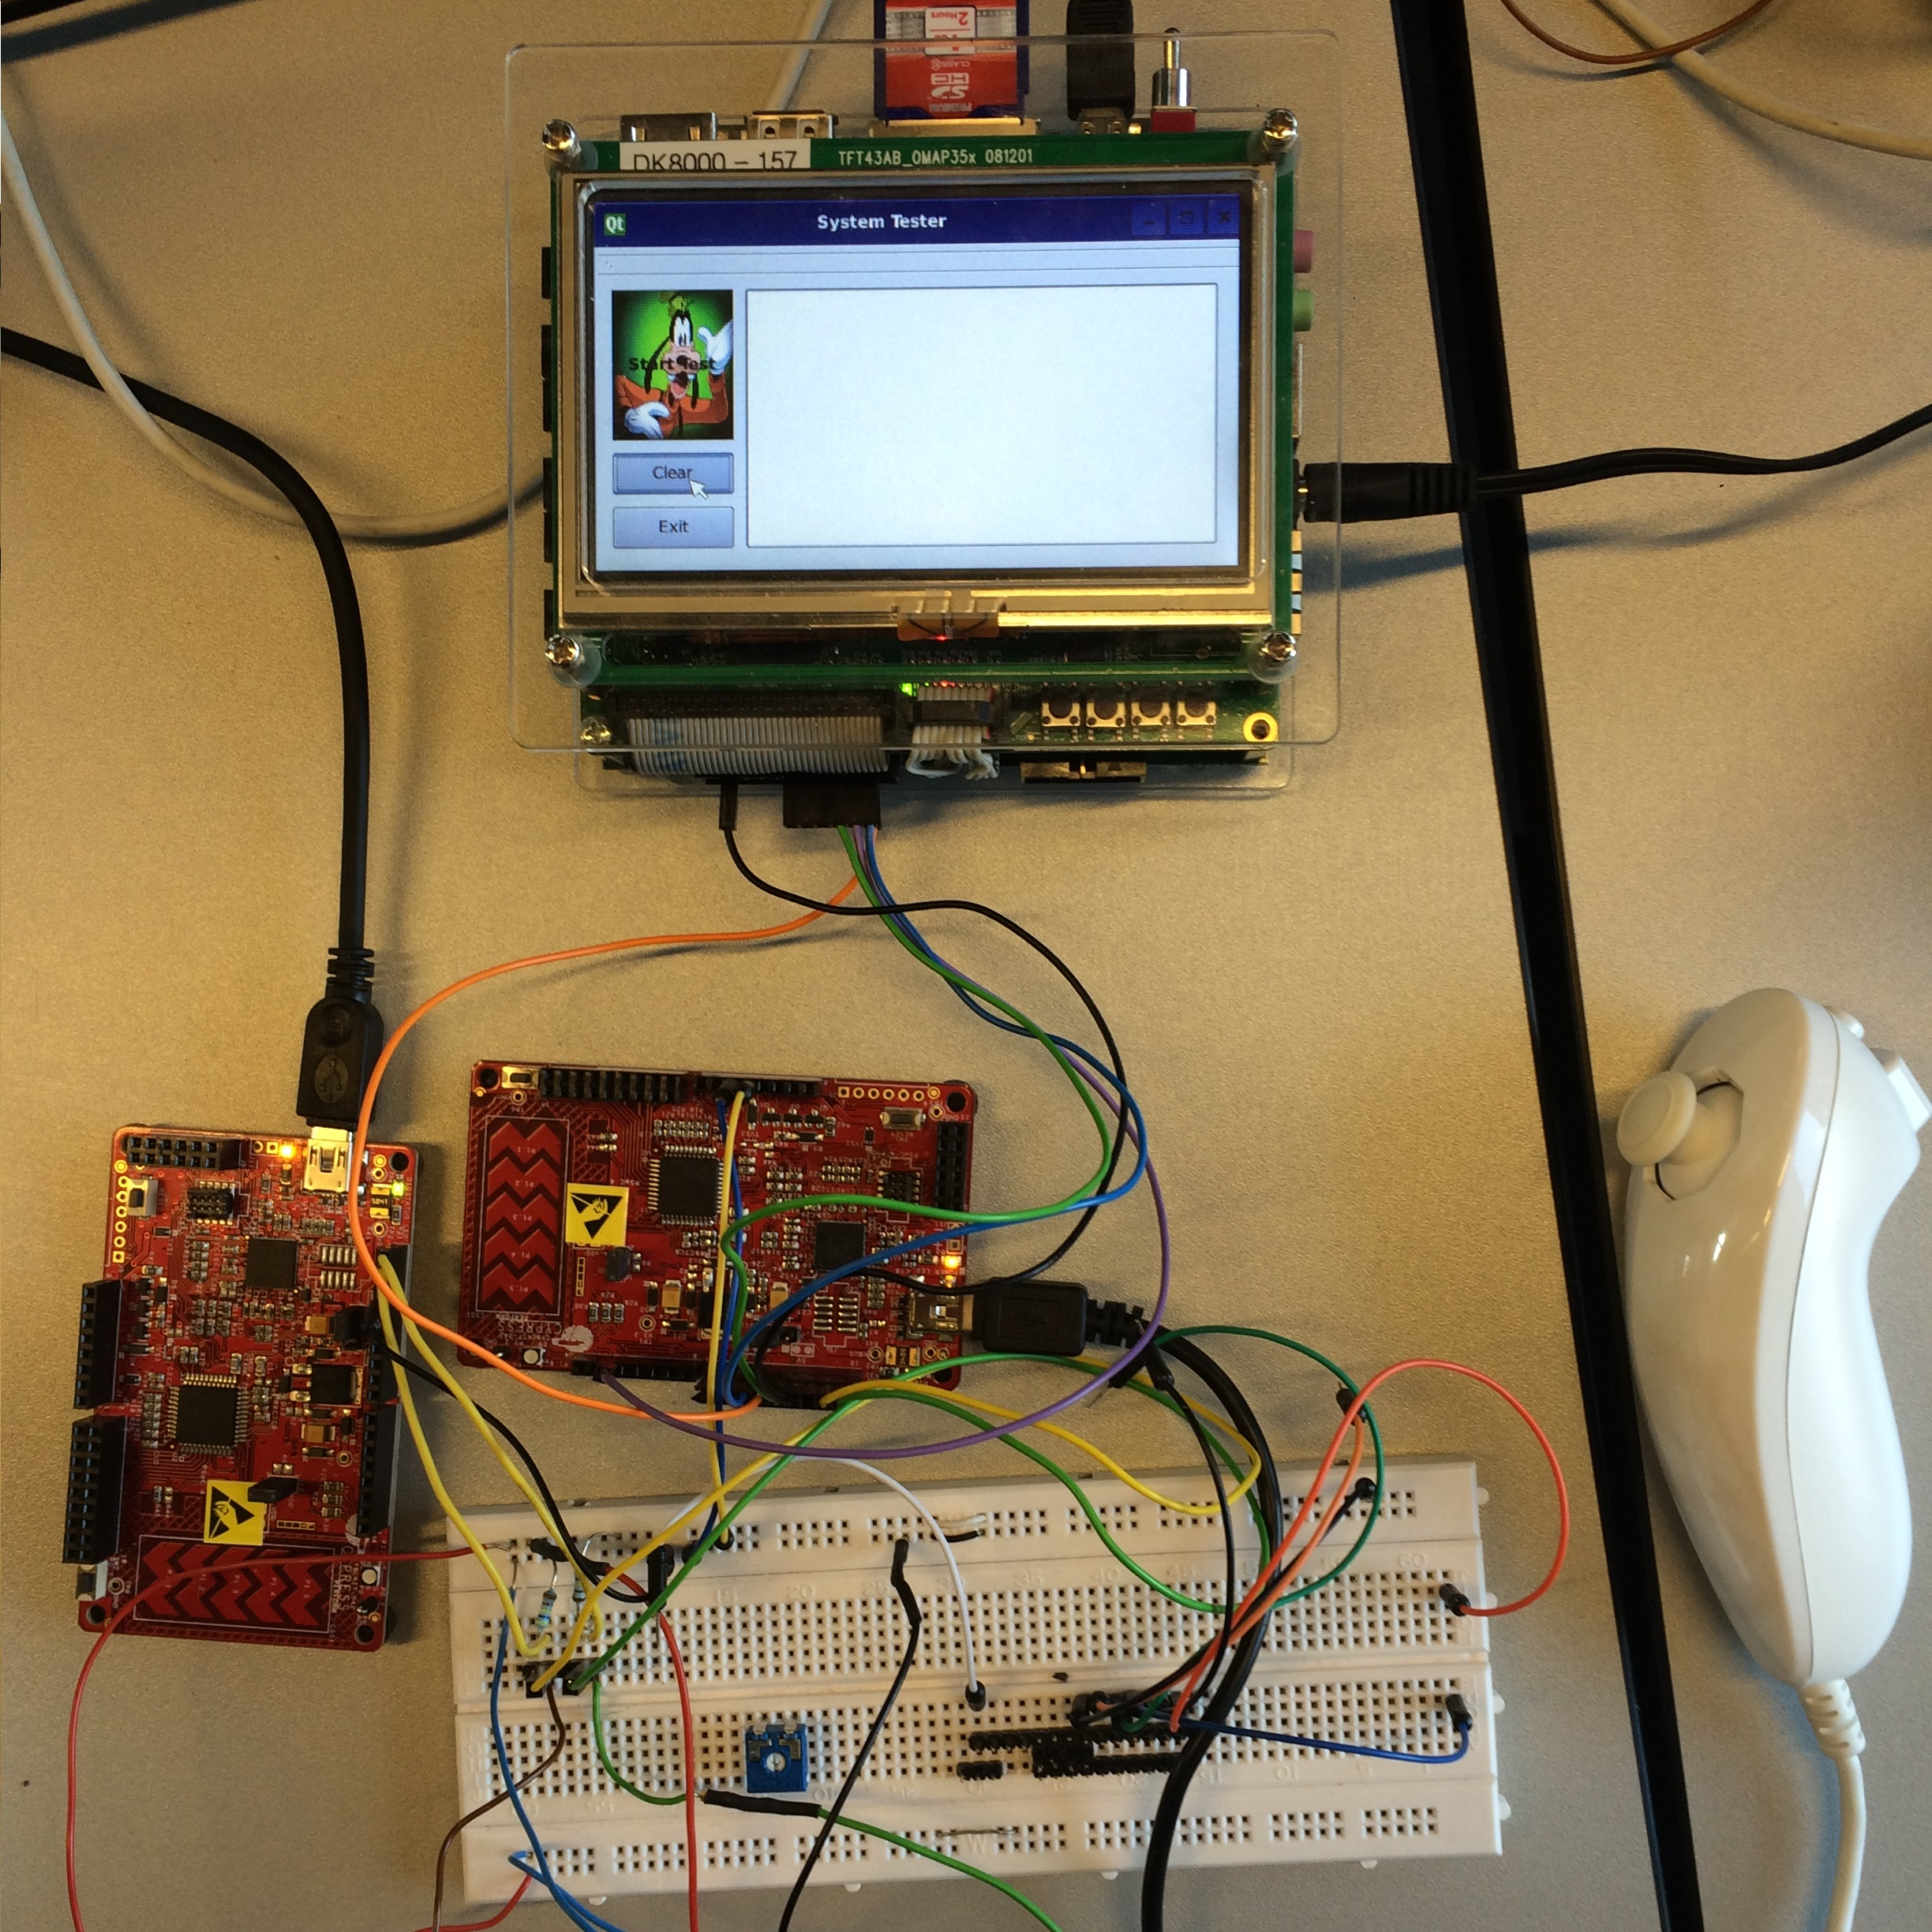
\includegraphics[width=\textwidth]{Test/images/IntegrationstestProtokoller/opstilling}
	\caption{Integrationstest opstilling}
	\label{figure:IntegrationstestOpstilling}
\end{figure}

Opstillingen viser, at Nunchuck'en og de to PSoC's er forbundet til samme I2C-netværk via fumlebrættet. PSoC0(PSoC'en til højre) er også forbundet til DevKit8000 via SPI, ledt igennem fumlebrættet. På Devkittet ses brugergrænsefladen, hvor testen initieres ved at klikke på "Start test". Brugergrænsefladen har også et terminalvindue, hvor testens status bliver udprintet.

Selve testen gennemføres, ved at der klikkes "Start test" på brugergrænsefladen, og derefter følges evt. instruktioner der vises på brugergrænsefladen. Det forventes, at efter testen, vil brugergrænsefladen fortælle, at testen blev gennemført uden fejl, og systemet er klar til brug. Figur \ref{figure:integrationstestresult} viser brugergrænsefladen efter endt system test.

\begin{figure}[H]
	\centering
	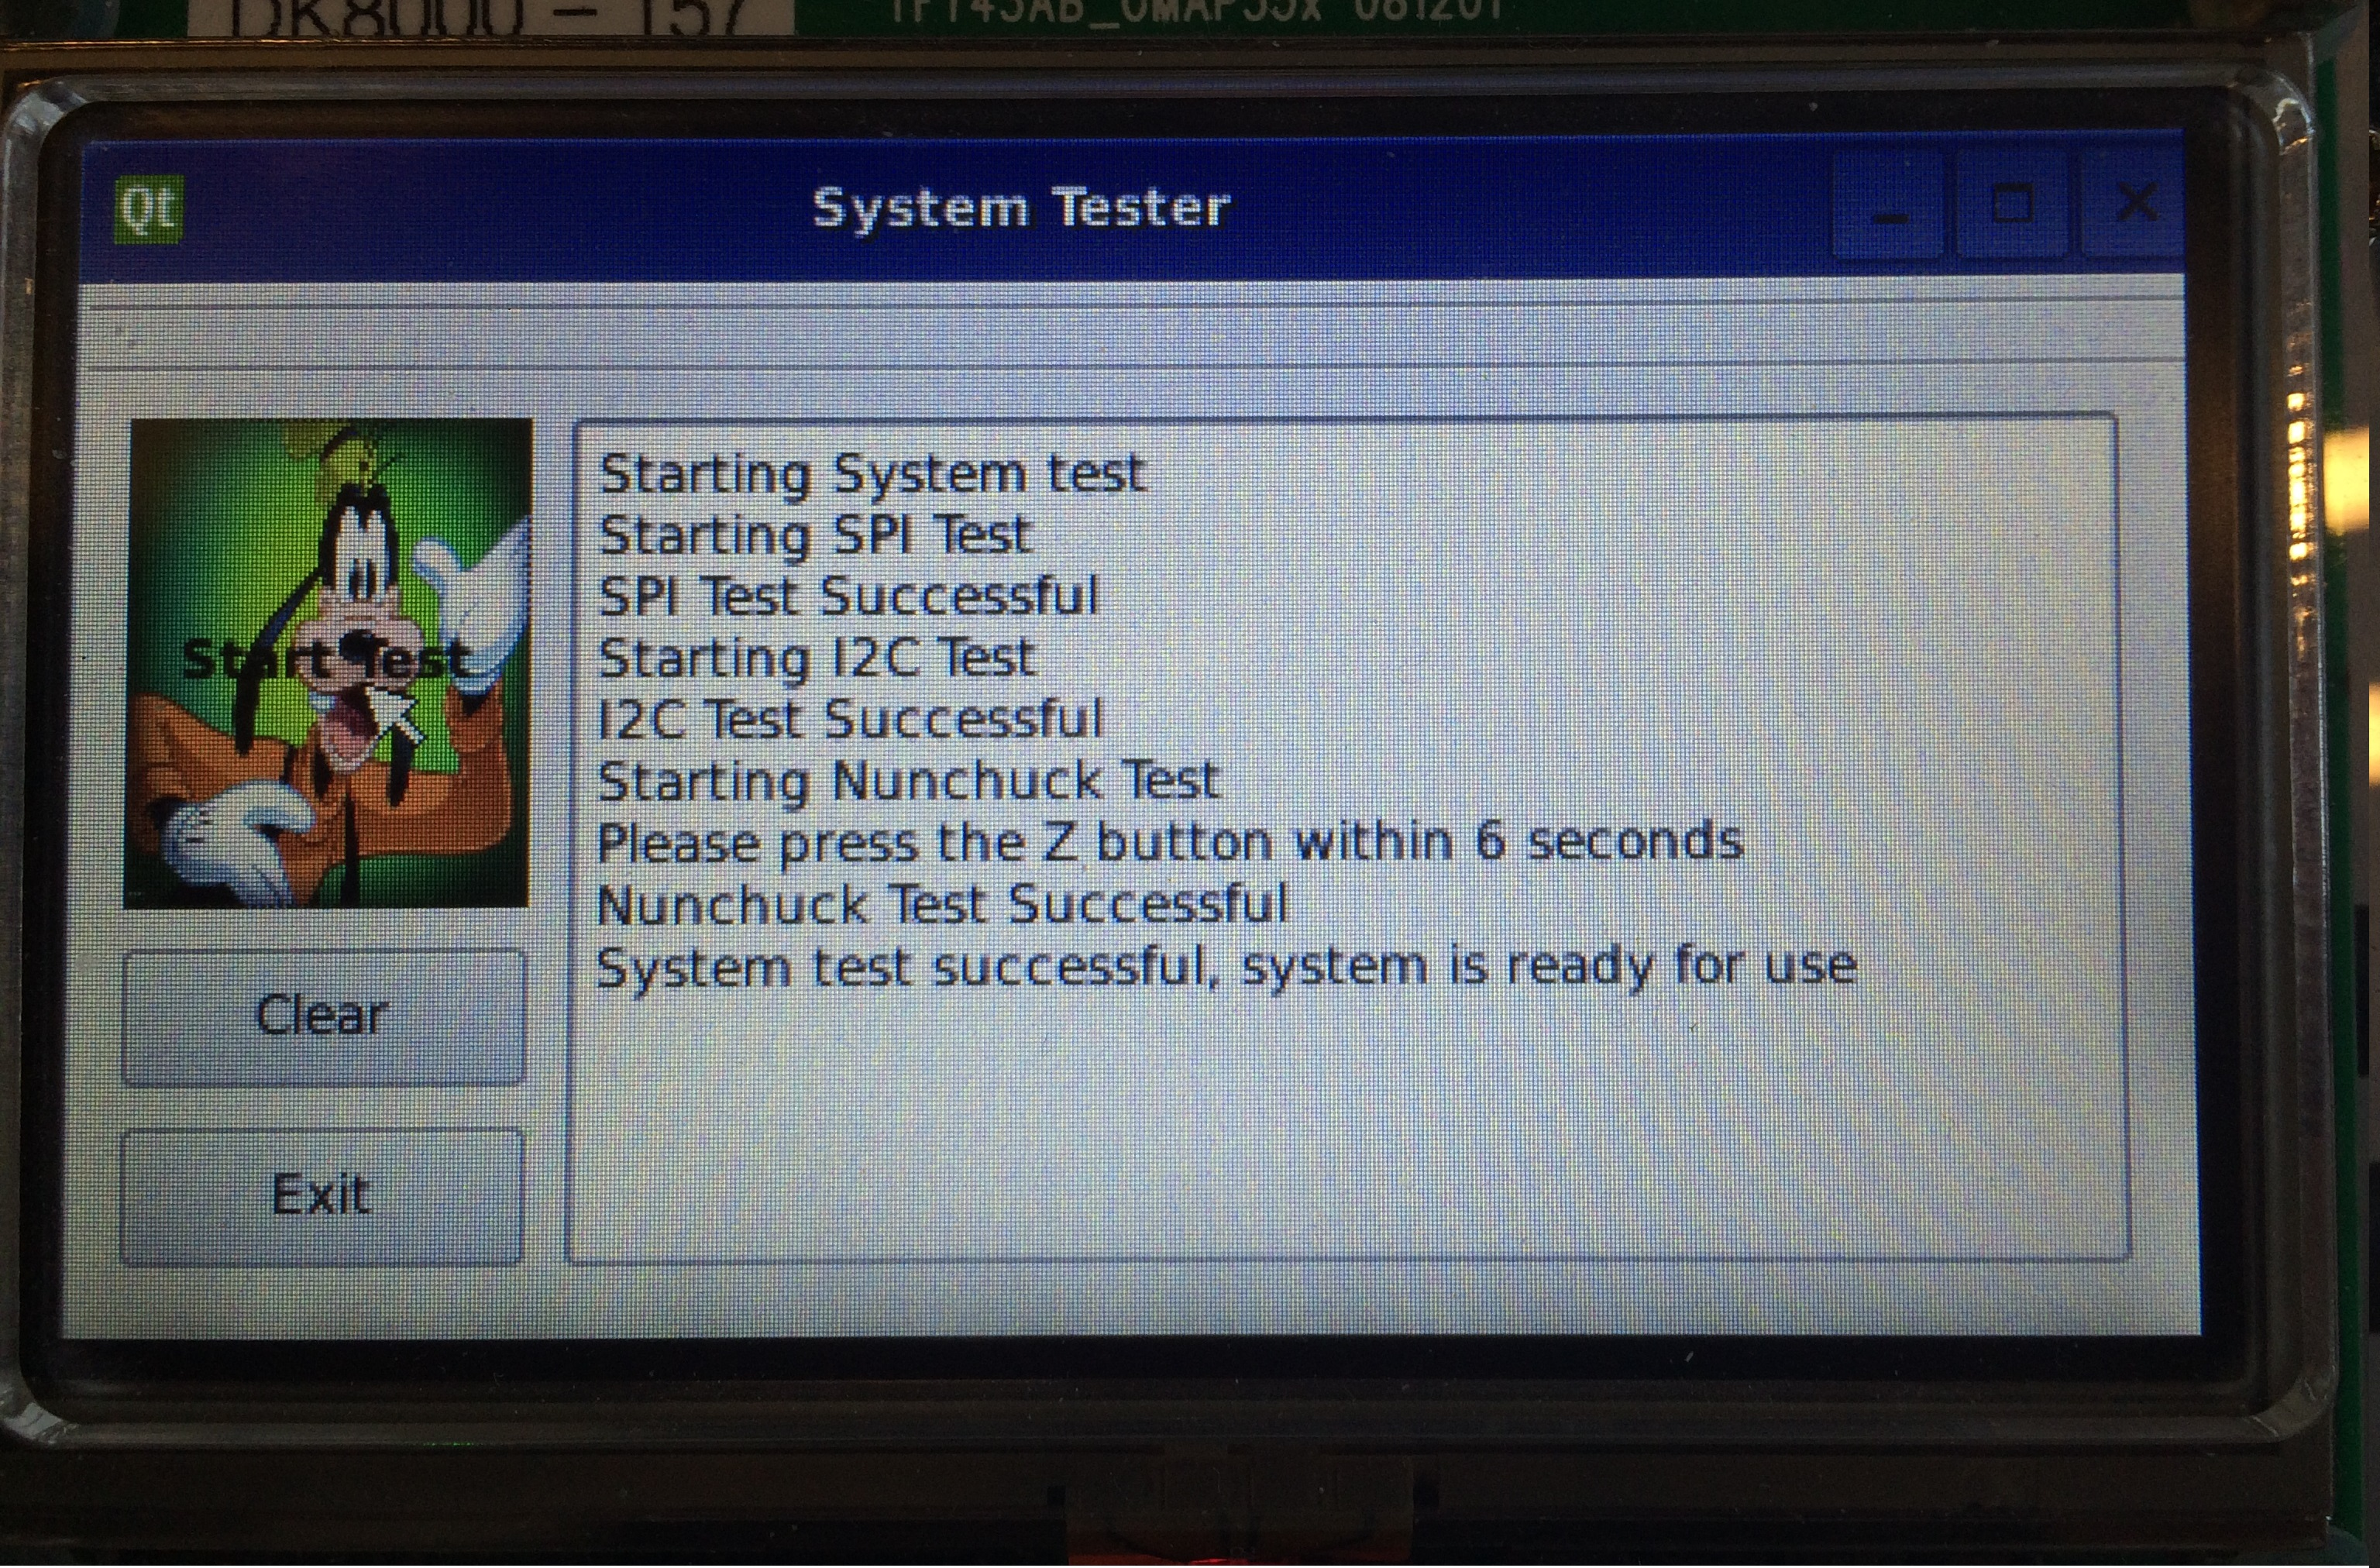
\includegraphics[width=\textwidth]{Test/images/IntegrationstestProtokoller/resultat2}
	\caption{Resultat af integrationstesten}
	\label{figure:integrationstestresult}
\end{figure}

Som det ses, er resultatet af testen som forventet, og testen er gennemført. Under testen bliver brugeren bedt om at trykke på nunchucken's 'z' knap. Hvis brugeren ikke klikker på knappen indenfor det angivne stykke tid, forventes det at testen vil fejle. Figur \ref{figure:integrationstestresult1} viser netop dette.


\begin{figure}[H]
	\centering
	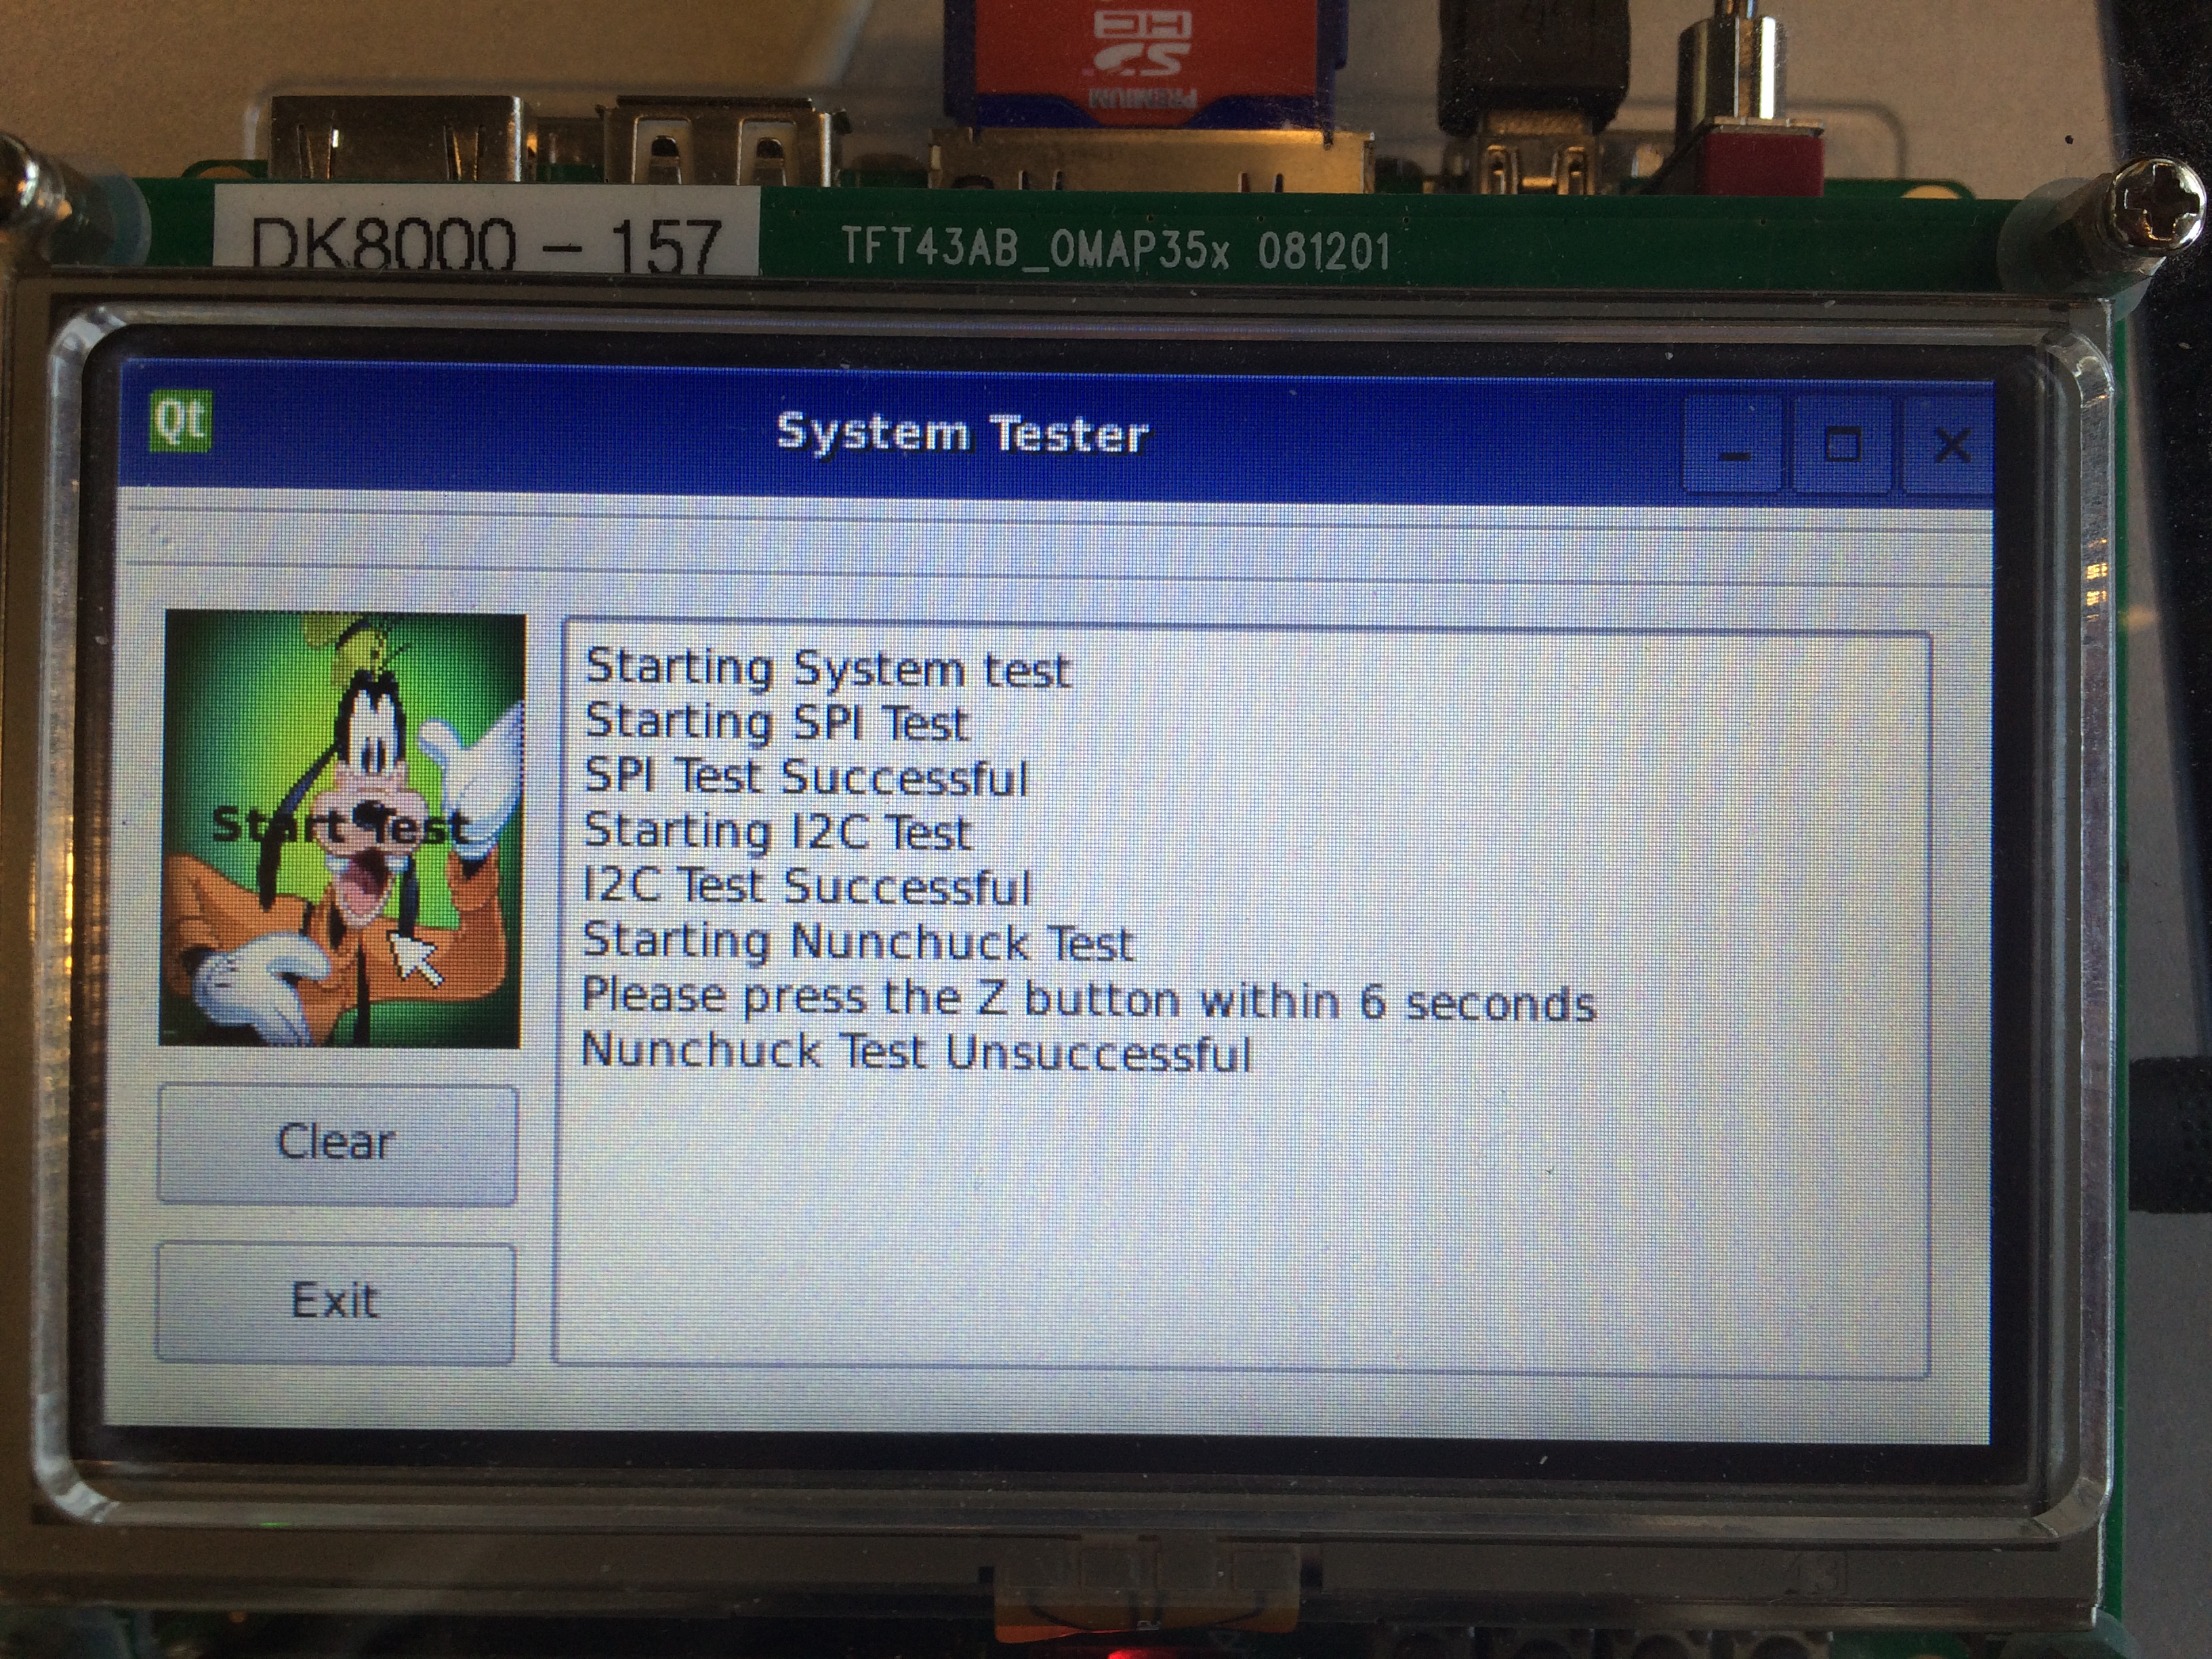
\includegraphics[width=\textwidth]{Test/images/IntegrationstestProtokoller/resultat1}
	\caption{Resultat hvis man ikke klikker på nunchuck}
	\label{figure:integrationstestresult1}
\end{figure}

Som det ses, fejlede testen, hvilket stemte overens med det forventede resultat. Derved kan det konkluderes at systemet opfører sig som forventet.

\section{Accepttest}